\documentclass{report}
% Include all project wide packages here.
\usepackage{fullpage}
\usepackage[style=ieee]{biblatex}
\usepackage[dutch]{babel}

\renewcommand{\familydefault}{\sfdefault}

\setmainfont[Ligatures=TeX]{Myriad Pro}
\setmathfont{Asana Math}
\setmonofont{Lucida Console}

\usepackage{titlesec, blindtext, color}
\definecolor{gray75}{gray}{0.75}
\newcommand{\hsp}{\hspace{20pt}}
\titleformat{\chapter}[hang]{\Huge\bfseries}{\thechapter\hsp\textcolor{gray75}{|}\hsp}{0pt}{\Huge\bfseries}
\renewcommand{\familydefault}{\sfdefault}
\renewcommand{\arraystretch}{1.2}
\setlength\parindent{0pt}

%For code listings
\definecolor{black}{rgb}{0,0,0}
\definecolor{browntags}{rgb}{0.65,0.1,0.1}
\definecolor{bluestrings}{rgb}{0,0,1}
\definecolor{graycomments}{rgb}{0.4,0.4,0.4}
\definecolor{redkeywords}{rgb}{1,0,0}
\definecolor{bluekeywords}{rgb}{0.13,0.13,0.8}
\definecolor{greencomments}{rgb}{0,0.5,0}
\definecolor{redstrings}{rgb}{0.9,0,0}
\definecolor{purpleidentifiers}{rgb}{0.01,0,0.01}


\lstdefinestyle{csharp}{
language=[Sharp]C,
showspaces=false,
showtabs=false,
breaklines=true,
showstringspaces=false,
breakatwhitespace=true,
escapeinside={(*@}{@*)},
columns=fullflexible,
commentstyle=\color{greencomments},
keywordstyle=\color{bluekeywords}\bfseries,
stringstyle=\color{redstrings},
identifierstyle=\color{purpleidentifiers},
basicstyle=\ttfamily\small}

\lstdefinestyle{c}{
language=C,
showspaces=false,
showtabs=false,
breaklines=true,
showstringspaces=false,
breakatwhitespace=true,
escapeinside={(*@}{@*)},
columns=fullflexible,
commentstyle=\color{greencomments},
keywordstyle=\color{bluekeywords}\bfseries,
stringstyle=\color{bluestrings},
identifierstyle=\color{purpleidentifiers}
}

\lstdefinestyle{vhdl}{
language=VHDL,
showspaces=false,
showtabs=false,
breaklines=true,
showstringspaces=false,
breakatwhitespace=true,
escapeinside={(*@}{@*)},
columns=fullflexible,
commentstyle=\color{greencomments},
keywordstyle=\color{bluekeywords}\bfseries,
stringstyle=\color{redstrings},
identifierstyle=\color{purpleidentifiers}
}

\lstdefinestyle{xaml}{
language=XML,
showspaces=false,
showtabs=false,
breaklines=true,
showstringspaces=false,
breakatwhitespace=true,
escapeinside={(*@}{@*)},
columns=fullflexible,
commentstyle=\color{greencomments},
keywordstyle=\color{redkeywords},
stringstyle=\color{bluestrings},
tagstyle=\color{browntags},
morestring=[b]",
  morecomment=[s]{<?}{?>},
  morekeywords={xmlns,version,typex:AsyncRecords,x:Arguments,x:Boolean,x:Byte,x:Char,x:Class,x:ClassAttributes,x:ClassModifier,x:Code,x:ConnectionId,x:Decimal,x:Double,x:FactoryMethod,x:FieldModifier,x:Int16,x:Int32,x:Int64,x:Key,x:Members,x:Name,x:Object,x:Property,x:Shared,x:Single,x:String,x:Subclass,x:SynchronousMode,x:TimeSpan,x:TypeArguments,x:Uid,x:Uri,x:XData,Grid.Column,Grid.ColumnSpan,Click,ClipToBounds,Content,DropDownOpened,FontSize,Foreground,Header,Height,HorizontalAlignment,HorizontalContentAlignment,IsCancel,IsDefault,IsEnabled,IsSelected,Margin,MinHeight,MinWidth,Padding,SnapsToDevicePixels,Target,TextWrapping,Title,VerticalAlignment,VerticalContentAlignment,Width,WindowStartupLocation,Binding,Mode,OneWay,xmlns:x}
}

%defaults
\lstset{
basicstyle=\ttfamily\small,
extendedchars=false,
numbers=left,
numberstyle=\ttfamily\tiny,
stepnumber=1,
tabsize=4,
numbersep=5pt
}
\addbibresource{../../library/bibliography.bib}

\title{EPO-2: Mid-term Design Report - Probleemstelling}
\author{Tijmen Witte}

\begin{document}

\chapter{Probleemstelling}
\label{ch:probleemstelling}

\section{Projectopgave: Mijnen-ontwijkende robot}

Het is de bedoeling dat er tijdens het EPO-2 project “Smart Robot Challenge” een autonome robot wordt ontworpen die zijn weg kan vinden over een veld dat bestaat uit zwarte lijnen op een witte ondergrond.
Vervolgens worden op het veld op nog onbekende plaatsen mijnen geplaatst, die de robot dient te ontwijken.
Als laatste wordt er nog één mijn toegevoegd, die op dat moment gevonden moet worden en dienst doet als schat.
Dit alles dient te worden voltooid door middel van zelfgemaakte VHDL en C-codes, die de directe besturing van de robot realiseren.


\section{Beschikbare infrastructuur}
\subsection{Spartan-3 robotplatform}

De basisvorm van de robot is van te voren gebouwd en bestaat uit een plateau waarop één Xilinx BASYS2 Spartan3E FPGA-bord is gemonteerd.
Op de FPGA worden hardwaremodules (de mijndetector) geïmplementeerd die door ons worden ontworpen.
Voor communicatie is er een XBee-module aanwezig.
Deze vormen samen de digitale besturing van de servomotoren die aan de onderkant van het plateau zitten.
Verder zijn er aan de onderkant ook nog lichtgevoelige sensors die de lijn detecteren, zodat deze gevolgd kan worden door de robot.

\begin{figure}[H]
	\centering
	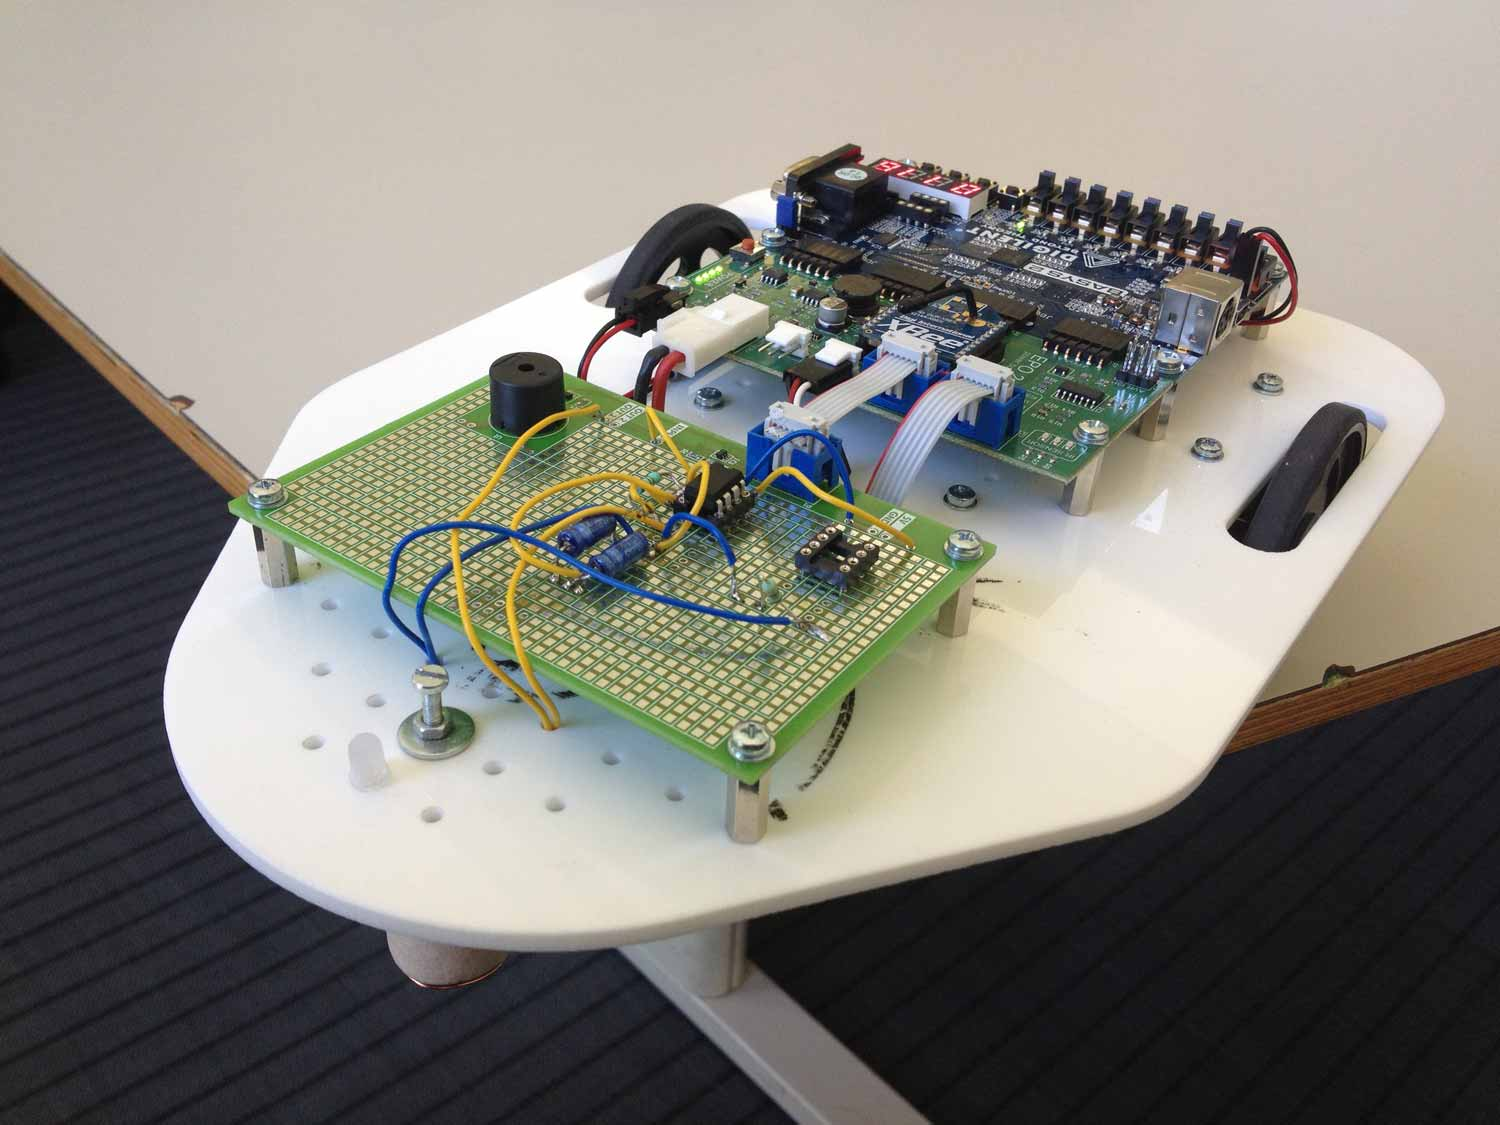
\includegraphics[width=0.6\textwidth]{robot.jpg}
	\caption{De robot die wij hebben gebruikt}
	\label{fig:robot}
\end{figure}






\subsection{Eigenschappen mijnenveld}

Het veld dat gebruikt wordt voor de robotcompetitie bestaat uit een zwart-wit geprint papiervel, dat bevestigd is op een houten bord met afmetingen 244 cm x 244 cm.
Het zwarte patroon wordt gevormd door een 5 bij 5 rooster van wegen en kruispunten.
De wegen zijn aangegeven als een zwarte strip van 15 mm breed, één wegsegment is 48cm lang.
In het midden van elk wegsegment zit een zwarte stip met een diameter van 30mm, deze dienen als de plaats waar de mijnen op komen te liggen.
De mijnen zijn gemaakt van zwartgeverfde verzinkte stalen ringen.
Aan elke zijde van het vierkante veld zijn er drie ingangswegen (16 cm lang) die aangegeven worden met de getallen 1 t/m 12.


\begin{figure}[H]
	\centering
	\includegraphics[width=0.6\textwidth]{competitionField2440x2440-rc.pdf}
	\caption{Het wedstrijdveld te gebruiken bij EPO-2}
	\label{fig:field}
\end{figure}


\section{Functionele eisen}

Aan de volgende functionele eisen moet de robot voldoen;

\begin{itemize}

\item
De robot moet een lijn kunnen volgen.


\item 
De robot moet een route kunnen volgen.

\item
De robot moet een mijn kunnen detecteren, onthouden waar deze ligt en vervolgens de mijn ontwijken.

\item 
De robot moet kunnen communiceren met de computer en andersom.

\end{itemize}

\newpage
\section{Randvoorwaarden}

De robot heeft een aantal eisen waaraan voldaan moet worden;

\begin{itemize}

\item
De robot in een fictieve box passen die niet groter is dan 30 cm x 25 cm x 20 cm.

\item
De robot mag maximaal 1 kg wegen.

\item
De aandrijving wordt gerealiseerd met behulp van elektromotoren en een batterij.
De batterij is de enige aanwezige energiebron op de robot.

\item
De robotaansturing kan alleen worden gedaan via de beschikbare Basys2 ontwikkelbord, die bestaat uit;

\begin{itemize}

\item
één Spartan-3 FPGA chip,

\item
twee XBee modules,

\item
één besturingsprogamma op een laptop dat geschreven is in de programmeertaal C.


\end{itemize}

\item
De FPGA-chip kan alleen werken met een VHDL-geschreven code.

\item
Het niet toegestaan om in het besturingsprogramma in te voeren waar de obstakels(mijnen) op het wedstrijdveld liggen 

\item
De robot moet zo gebouwd zijn dat deze geen schade of markeringen kan aanbrengen aan het wedstrijdveld.

\end{itemize}

\section{Plan van aanpak}

Er is door zes personen aan het EPO-2 project “Smart Robot Challenge” gewerkt, dit gebeurde in zaal 1.060 aan de Drebbelweg 5.
Aan de hand van verschillende Just-in-time trainingen worden in de loop van het project de onderdelen voor de robot beter bestudeerd en vervolgens ontworpen en gemaakt.
Daarnaast zijn er nog tutorials waarin benodigde kennis wordt uitgelegd.
Een uitgebreid plan van aanpak is te vinden in bijlage \ref{sec:pva}.

\end{document}